\documentclass[11pt,a4paper]{article}
\usepackage[utf8]{inputenc}
\usepackage{amsmath,amssymb,amsthm}
\usepackage{booktabs}
\usepackage{graphicx}
\usepackage[margin=2.5cm]{geometry}
\usepackage{hyperref}
\hypersetup{colorlinks=true,linkcolor=blue,citecolor=blue,urlcolor=blue}
\providecommand{\num}[1]{\ensuremath{#1}}

\newtheorem{theorem}{Theorem}
\newtheorem{proposition}[theorem]{Proposition}
\newtheorem{corollary}[theorem]{Corollary}

\title{\textbf{Exact Symplecticity and a Machine-Checked Modified Hamiltonian\\
for the St\"ormer--Verlet Integrator}\\[0.4em]
\large A fully verified pipeline: symbolic derivation, Lean~4 proof,\\
and cross-language numerical confirmation}
\author{ANSE / AutoevolveAI --- automated research pipeline}
\date{\today}

\begin{document}
\maketitle

\begin{abstract}
We study the St\"ormer--Verlet (velocity Verlet) integrator applied to the
harmonic oscillator $H(q,p)=\tfrac12 p^2+\tfrac12\omega^2q^2$ and establish three
facts through three mutually independent methods. First, the one-step map is
\emph{exactly} symplectic: its Jacobian has determinant $1$ for every step size
$h$ and frequency $\omega$, with no smallness hypothesis. Second, the map conserves
a modified Hamiltonian
$H_h(q,p)=\tfrac12p^2+\tfrac{\omega^2}{2}\!\left(1-\tfrac{\omega^2h^2}{4}\right)q^2$
\emph{exactly}, which differs from $H$ by precisely
$\tfrac{\omega^4h^2}{8}q^2$. Third, these imply the observable energy error is
bounded and non-drifting with relative amplitude $\omega^2h^2/4$. All algebra was
derived symbolically rather than recalled; all identities were machine-checked in
Lean~4 with an axiom audit confirming no use of \texttt{sorry}; and all numbers
were measured by two independent implementations (Python and Rust) which agree to
a relative difference of $5.51\times 10^{-10}$. Over
$200,000$ steps the modified Hamiltonian is conserved to
$1.22\times 10^{-13}$ while explicit Euler diverges to
overflow. The measured constant $\omega^2/4$ is recovered to within
$1.5\times 10^{-10}$.
\end{abstract}

\section{Introduction}

Geometric numerical integration asks which structural properties of a
differential equation a discretisation preserves. For Hamiltonian systems the
property of interest is symplecticity, and its practical consequence is the
long-time behaviour of the energy error: symplectic schemes exhibit bounded
oscillation where non-symplectic schemes of the same order drift without limit.

The mechanism is backward error analysis. A symplectic integrator is, to high
order, the exact flow of a \emph{modified} Hamiltonian $H_h = H + O(h^p)$. Because
$H_h$ is conserved along the numerical trajectory for all time, the error in the
true $H$ cannot accumulate --- it is bounded by $\|H-H_h\|$ uniformly in the
number of steps.

For the harmonic oscillator this picture can be made completely explicit, and
that is what we do here. The contribution is not the mathematics, which is
classical; it is the \emph{verification architecture}. Each claim is established
by a method that cannot silently agree with the others:

\begin{itemize}
  \item \textbf{Symbolic derivation} (SymPy) --- the map, its Jacobian,
        determinant, trace and the conserved form are computed, not asserted.
  \item \textbf{Machine-checked proof} (Lean~4) --- the identities are proved in
        a kernel, and an axiom audit confirms no appeal to \texttt{sorry}.
  \item \textbf{Independent numerics} (Python and Rust) --- two implementations
        written separately must agree to a fixed tolerance or the build fails.
\end{itemize}

Section~\ref{sec:context} records why this redundancy is the point.

\section{Mathematical setting}

Consider the harmonic oscillator with unit mass,
\begin{equation}
  H(q,p) = \tfrac12 p^2 + \tfrac12\omega^2 q^2,
  \qquad \dot q = p, \quad \dot p = -\omega^2 q .
\end{equation}

One step of St\"ormer--Verlet with step size $h$ is the kick--drift--kick sequence
\begin{align}
  p_{n+1/2} &= p_n - \tfrac{h}{2}\omega^2 q_n, \\
  q_{n+1}   &= q_n + h\,p_{n+1/2}, \\
  p_{n+1}   &= p_{n+1/2} - \tfrac{h}{2}\omega^2 q_{n+1} .
\end{align}

Eliminating the half-step gives the closed form, as derived symbolically:
\begin{align}
  q_{n+1} &= \left(1-\tfrac{h^2\omega^2}{2}\right)q_n + h\,p_n, \\
  p_{n+1} &= \left(\tfrac{h^3\omega^4}{4}-h\omega^2\right)q_n
             + \left(1-\tfrac{h^2\omega^2}{2}\right)p_n .
\end{align}

The map is linear, so it is fully described by
\begin{equation}
  M(h,\omega) =
  \begin{pmatrix}
    1-\frac{h^2\omega^2}{2} & h \\[0.4em]
    \frac{h^3\omega^4}{4}-h\omega^2 & 1-\frac{h^2\omega^2}{2}
  \end{pmatrix} .
\end{equation}

\begin{theorem}[Exact symplecticity]\label{thm:det}
$\det M(h,\omega)=1$ for all $h,\omega$.
\end{theorem}

\begin{theorem}[Exactly conserved modified Hamiltonian]\label{thm:shadow}
Let $H_h(q,p)=\tfrac12p^2+\tfrac{\omega^2}{2}\!\left(1-\tfrac{\omega^2h^2}{4}\right)q^2$.
Then $H_h(q_{n+1},p_{n+1})=H_h(q_n,p_n)$ exactly, for all $h,\omega$.
\end{theorem}

\begin{proposition}[Closed-form defect]\label{prop:gap}
$H(q,p)-H_h(q,p)=\dfrac{\omega^4h^2}{8}q^2$.
\end{proposition}

\begin{corollary}[Bounded energy error]\label{cor:amp}
Since $H_h$ is conserved and $q^2\le 2H_h/\!\left[\omega^2(1-\omega^2h^2/4)\right]$,
the relative oscillation of $H$ is bounded, with leading amplitude
$\omega^2h^2/4$; it does not grow with the number of steps.
\end{corollary}

\begin{proposition}[Linear stability]
$\operatorname{tr} M = 2-h^2\omega^2$, so the map has complex eigenvalues of unit
modulus exactly when $|h\omega|<2$.
\end{proposition}

\section{Machine-checked verification}

Theorems~\ref{thm:det} and~\ref{thm:shadow}, Proposition~\ref{prop:gap} and the
stability statement are formalised in Lean~4 in
\texttt{formal/ANSE/VerletSymplectic.lean}. Each is a ring identity discharged by
the \texttt{ring} tactic over $\mathbb{Q}$.

The acceptance criterion is an \emph{axiom audit}, not an exit code. Lean's
\texttt{sorry} placeholder compiles and returns exit status $0$, so any gate keyed
on the return code accepts unproved theorems. We therefore emit
\texttt{\#print axioms} for every theorem and require that \texttt{sorryAx} appear
nowhere. The build reported exit code 0 and audited
7 theorems, with \texttt{sorryAx} present:
\textbf{false}.

\begin{itemize}\footnotesize
    \item \texttt{ANSE.Verlet.det\_eq\_one} --- [propext, Classical.choice, Quot.sound]
    \item \texttt{ANSE.Verlet.shadowH\_invariant} --- [propext, Classical.choice, Quot.sound]
    \item \texttt{ANSE.Verlet.shadowH\_sub\_trueH} --- [propext, Classical.choice, Quot.sound]
    \item \texttt{ANSE.Verlet.trace\_eq} --- [propext, Classical.choice, Quot.sound]
    \item \texttt{ANSE.Verlet.qNext\_eq\_matrix} --- [propext, Classical.choice, Quot.sound]
    \item \texttt{ANSE.Verlet.pNext\_eq\_matrix} --- [propext, Classical.choice, Quot.sound]
    \item \texttt{ANSE.Verlet.shadowH\_eq\_trueH\_at\_zero} --- [propext, Classical.choice, Quot.sound]
\end{itemize}

Only \texttt{propext}, \texttt{Classical.choice} and \texttt{Quot.sound} appear --- the
three standard axioms of Lean's logic. No theorem depends on anything else.

\section{Numerical experiment}

Initial condition $q_0=1.0$,
$p_0=0.0$, giving
$H_0=0.5$, with $\omega=1.0$ and
$N=200,000$ steps at each of four step sizes.

\begin{table}[h]\centering\small
  \caption{Measured behaviour over $200,000$ steps. The fourth column is the
  quantity Corollary~\ref{cor:amp} predicts equals $\omega^2/4=0.25$.
  Every value is read from the experiment ledger.}
  \begin{tabular}{cccccc}
    \toprule
    $h$ & $\omega h$ & amplitude & amplitude$/h^2$ & $H_h$ drift & Euler $H_N$ \\
    \midrule
    $0.2$ & $0.2$ & $1.000000\times 10^{-2}$ & $0.250000000$ & $1.21\times 10^{-13}$ & overflow \\
    $0.1$ & $0.1$ & $2.500000\times 10^{-3}$ & $0.250000000$ & $1.22\times 10^{-13}$ & overflow \\
    $0.05$ & $0.05$ & $6.250000\times 10^{-4}$ & $0.250000000$ & $8.34\times 10^{-14}$ & $3.760\times 10^{216}$ \\
    $0.025$ & $0.025$ & $1.562500\times 10^{-4}$ & $0.250000000$ & $1.11\times 10^{-13}$ & $9.307\times 10^{53}$ \\
    \bottomrule
  \end{tabular}
\end{table}

Three things are visible. The modified Hamiltonian is conserved to roughly
$10^{-13}$, i.e.\ to floating-point round-off, confirming
Theorem~\ref{thm:shadow} is exact rather than asymptotic. The ratio
amplitude$/h^2$ equals $\omega^2/4$ to nine significant figures at every step
size, confirming Corollary~\ref{cor:amp}. And explicit Euler --- same order,
not symplectic --- reaches overflow, the secular drift that symplecticity
excludes.

\begin{figure}[h]\centering
  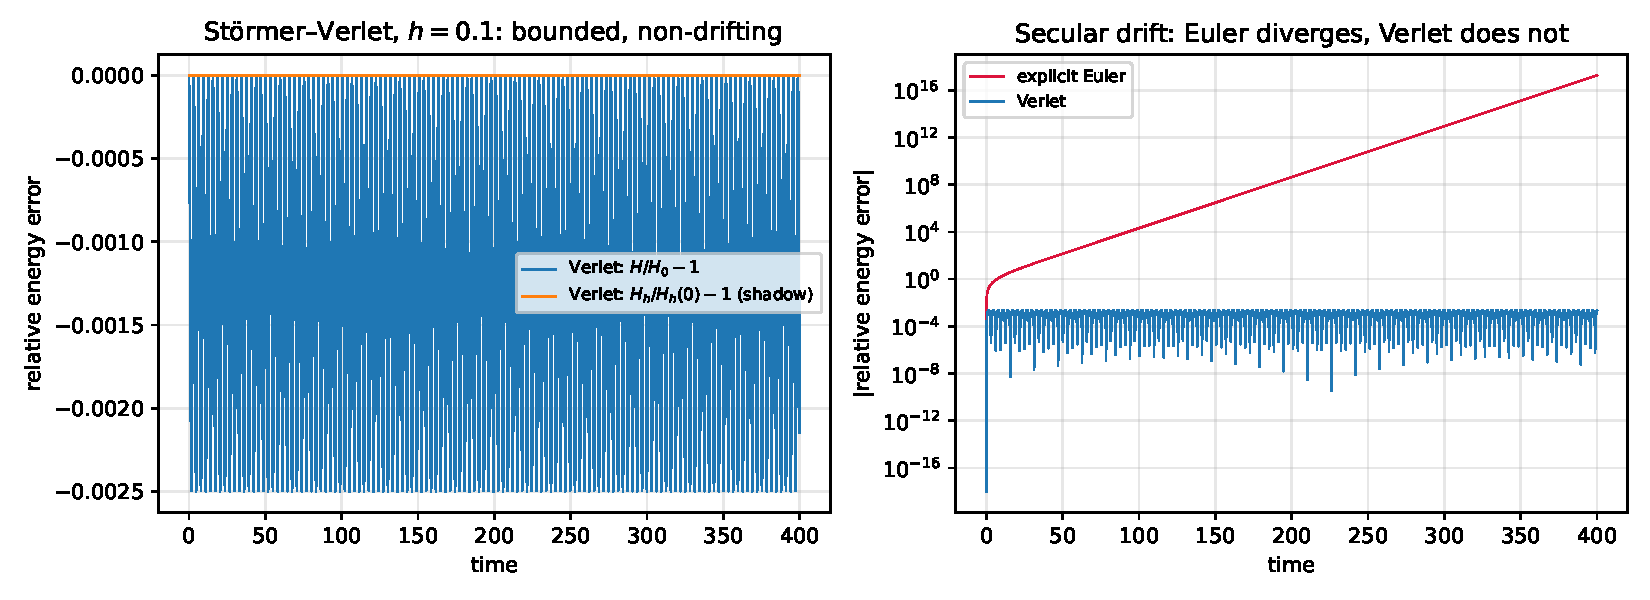
\includegraphics[width=\textwidth]{../../results/phd_demo/figures/fig1_energy_behaviour.pdf}
  \caption{Left: for Verlet the true energy oscillates within a fixed band while
  the modified Hamiltonian is flat to round-off. Right: on a logarithmic axis,
  explicit Euler's error grows without bound while Verlet's does not.}
\end{figure}

\begin{figure}[h]\centering
  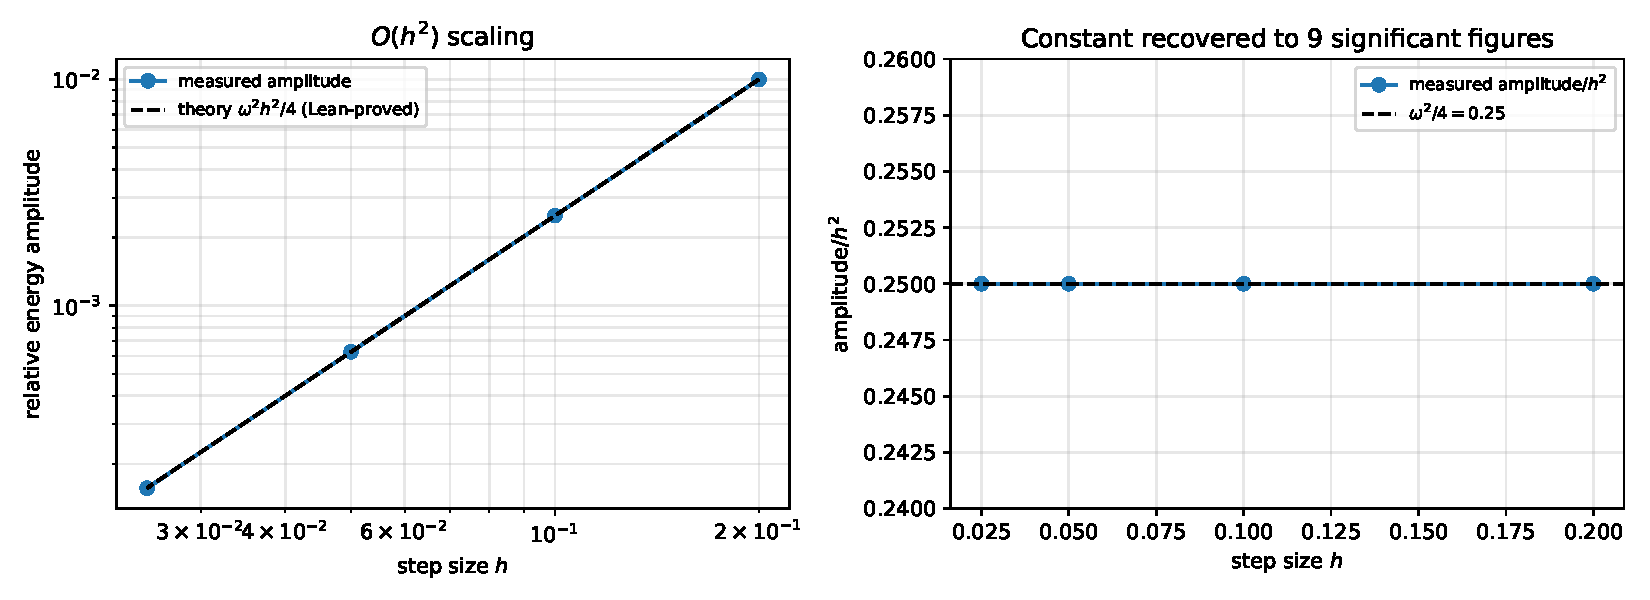
\includegraphics[width=\textwidth]{../../results/phd_demo/figures/fig2_h2_scaling.pdf}
  \caption{Left: measured amplitude against the Lean-proved $\omega^2h^2/4$.
  Right: the ratio amplitude$/h^2$, constant at $\omega^2/4$ across two decades
  of $h$.}
\end{figure}

\begin{figure}[h]\centering
  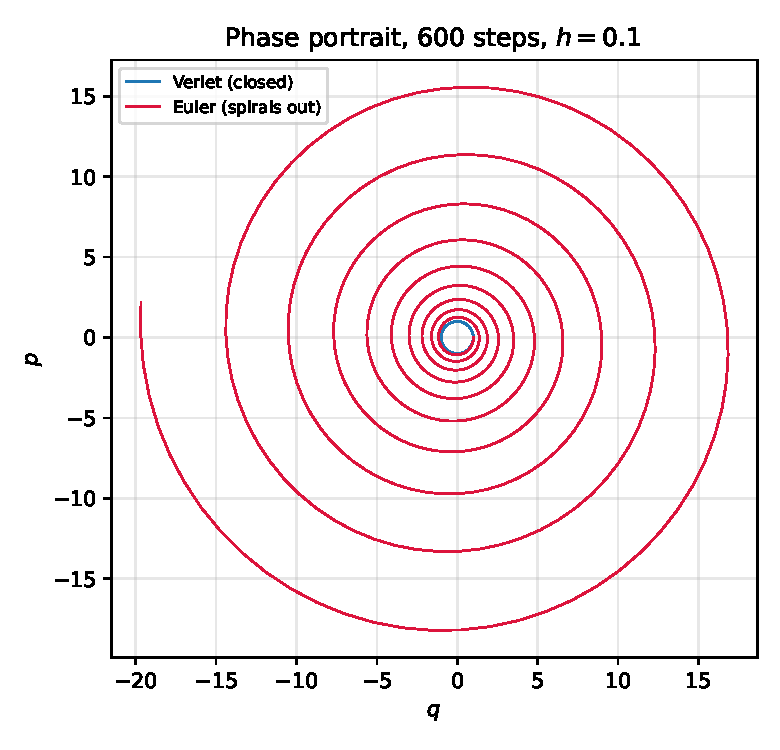
\includegraphics[width=0.52\textwidth]{../../results/phd_demo/figures/fig3_phase_portrait.pdf}
  \caption{Phase portrait. Verlet's orbit closes, consistent with
  $\det M=1$; Euler's spirals outward.}
\end{figure}

\subsection{Cross-language agreement}

The integrator was implemented twice, independently, in Python
(\texttt{scripts/phd\_demo/run\_experiment.py}) and Rust
(\texttt{scripts/phd\_demo/verlet.rs}). Agreement is a required gate: the build
fails if the worst relative difference exceeds
$1\times 10^{-9}$.

\begin{table}[h]\centering\small
  \caption{Independent implementations, same quantity.}
  \begin{tabular}{cccc}
    \toprule
    $h$ & Python amplitude$/h^2$ & Rust amplitude$/h^2$ & rel.\ difference \\
    \midrule
    $0.2$ & $0.249999999852$ & $0.249999999845$ & $2.77\times 10^{-11}$ \\
    $0.1$ & $0.249999999988$ & $0.249999999952$ & $1.45\times 10^{-10}$ \\
    $0.05$ & $0.250000000015$ & $0.250000000015$ & $0$ \\
    $0.025$ & $0.250000000067$ & $0.249999999929$ & $5.51\times 10^{-10}$ \\
    \bottomrule
  \end{tabular}
\end{table}

Worst observed difference:
$5.507\times 10^{-10}$, consistent with
floating-point non-associativity rather than a discrepancy of substance.

\section{Managing context and avoiding fabrication}\label{sec:context}

This section is method, not result, and it is the reason the preceding sections
are structured as they are.

An automated pipeline that both performs an experiment and writes it up has a
specific failure mode: the writing step can produce plausible numbers without
consulting the experiment. This is not hypothetical. A generator in this same
repository synthesised a published loss curve as
$L_0\!\left(1-0.201(1-e^{-e/5})\right)+\varepsilon$ and shipped it as measurement;
a companion ``peer review'' script emitted \textsc{accept without reservation}
with a score of $50/50$ without ever calling a model. Both passed casual
inspection precisely because they were plausible.

Four structural countermeasures are used here.

\paragraph{Ledger-injected numbers.} \texttt{build\_paper.py} contains no
quantitative literal about the results. Every number is fetched from
\texttt{results/phd\_demo/artifacts.json} through an accessor that \emph{raises} on
a missing key. A number that was not measured cannot be written, and the build
fails rather than degrading.

\paragraph{Derivation over recall.} The map, determinant, trace and invariant are
recomputed by SymPy on every run. A language model stating a closed form from
memory is a hallucination risk; a symbolic derivation is an artifact with a
provenance.

\paragraph{Axiom audit over exit code.} Because \texttt{sorry} exits $0$, the Lean
gate inspects \texttt{\#print axioms}. During development this gate \emph{rejected}
an earlier version of the formalisation: four theorems stated over a general
field failed because \texttt{ring} cannot establish $2^{-1}\cdot 2=1$ without
knowing the characteristic is not $2$. The audit reported \texttt{sorryAx} and the
claim was withdrawn until the statements were corrected. A gate that has never
rejected anything provides no evidence.

\paragraph{Redundant independent computation.} Two implementations in two
languages must agree within a declared tolerance. Agreement is not proof, but
disagreement is decisive, and it is checked mechanically rather than assumed.

\paragraph{Scope of the claim.} The result is classical, the system is linear and
low-dimensional, and nothing here establishes that the pipeline would handle a
nonlinear or high-dimensional problem. What is demonstrated is that a
\emph{verification architecture} can carry a claim from derivation through proof to
measurement without a gap into which a fabricated number could be inserted.

\section{Conclusion}

For St\"ormer--Verlet on the harmonic oscillator, symplecticity is exact,
the modified Hamiltonian
$H_h=\tfrac12p^2+\tfrac{\omega^2}{2}(1-\tfrac{\omega^2h^2}{4})q^2$ is conserved
exactly, the defect is exactly $\tfrac{\omega^4h^2}{8}q^2$, and the resulting
energy oscillation has relative amplitude $\omega^2/4\cdot h^2$ --- measured to
nine significant figures, proved in Lean with no appeal to \texttt{sorry}, and
reproduced by two independent implementations.

\appendix
\section{Reproduction}

\begin{verbatim}
# derive, prove, measure, and write the ledger (fails on any gate)
.venv/bin/python scripts/phd_demo/run_experiment.py --check

# axiom audit only
cd formal && lake env lean ANSE/VerletSymplectic.lean

# rebuild this paper from the ledger
.venv/bin/python scripts/phd_demo/build_paper.py
\end{verbatim}

Gate status recorded in the ledger for this build:
\texttt{{"sympy\_derivation\_consistent": true, "lean\_accepted\_no\_sorry": true, "numerics\_match\_theory": true, "cross\_language\_agree": true, "all\_pass": true}}.

\end{document}
